With the verification of Moltres' neutronics modeling capabilities in the
context of the \gls{MSFR}, we now move on to the multiphysics simulation
results. This chapter covers the steady-state multiphysics simulation results
from Moltres.

The procedure for obtaining the steady-state results involved several steps
due to the highly coupled \glspl{PDE}. First, we ran a preliminary transient
simulation of fluid flow in the \gls{MSFR} core, starting from zero inlet
velocity and gradually ramping it up to match the nominal flow rate (4.5 m$^3$
s$^{-1}$); otherwise Moltres had difficulty converging to the desired fully
developed flow profile. We imposed a parabolic flow profile at the inlet.
Next, we imported these fully developed flow values as initial values for
velocity in the actual transient simulation modeling the full coupled
neutronics and thermal-hydraulics. The initial values for the temperature and
neutron group flux distributions are 953 K and $1 \times 10^{14}$ cm$^{-2}$
s$^{-1}$ uniformly throughout the geometry. Finally, we assume that steady
state is reached when the volume integral values of every variable remain
constant (up to 6 sig. fig.) for at least four seconds in the simulation; this
time period corresponds to the nominal circulation time of the \gls{MSFR}.

For a direct comparison with the steady-state results from the Polimi and
TUDelft models \cite{aufiero_development_2014}, we will first present our
steady-state results without modeling decay heat. After this comparison, we
separately discuss the minor differences borne from decay heat modeling in the
last subsection.

\section{Steady-State Thermal-Hydraulics Results}

\begin{figure}[t!]
    \centering
    \begin{subfigure}[t]{.365\textwidth}
        \centering
        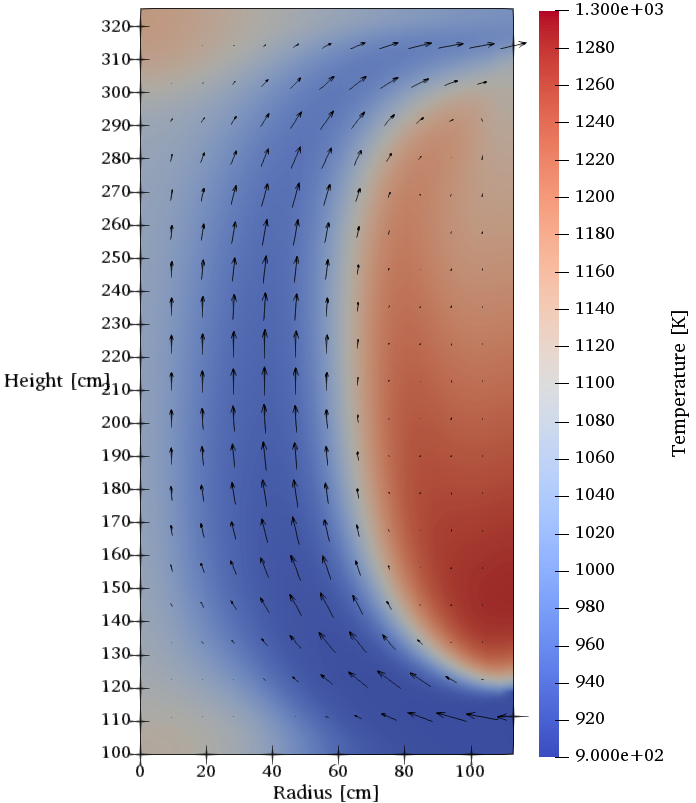
\includegraphics[width=\textwidth]{flow-temp}
    \end{subfigure}
    \hfill
    \begin{subfigure}[t]{.625\textwidth}
        \centering
        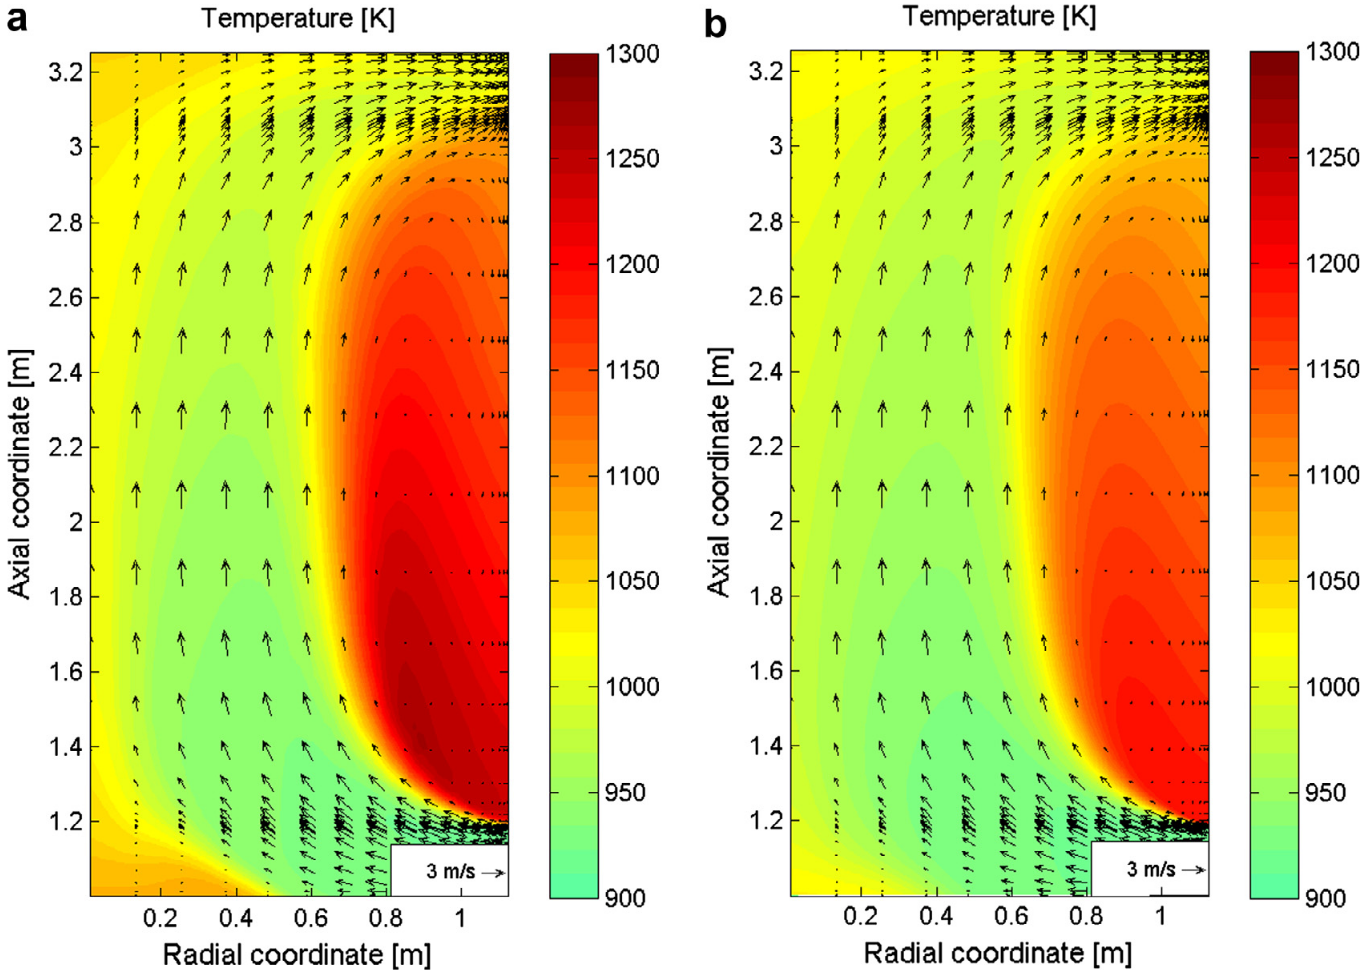
\includegraphics[width=\textwidth]{flow-temp-fiorina}
    \end{subfigure}
    \caption{Temperature and velocity fields in the core from Moltres
    (left), Polimi (center), and TUDelft (right) models. The colors represent
    temperature according to the respective colorbars while the arrows
    represent velocity fields.}
    \label{fig:flow-temp}
\end{figure}

\begin{figure}[t!]
    \centering
    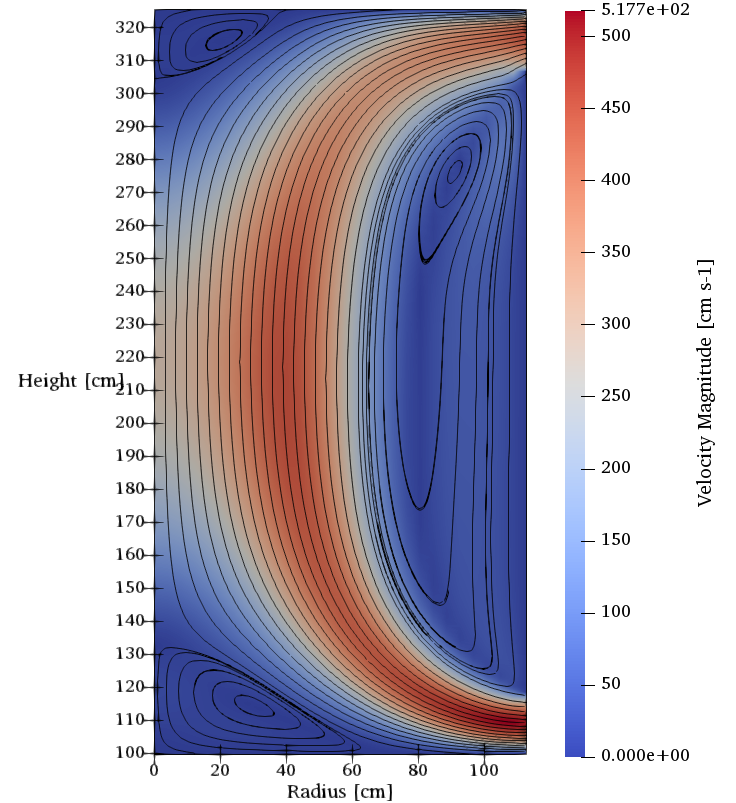
\includegraphics[width=.6\textwidth]{flow}
    \caption{Fuel salt flow streamlines and velocity magnitude in the core.
    The colors represent velocity magnitude according to the colorbar on the
    right.}
    \label{fig:flow}
\end{figure}

Figure \ref{fig:flow-temp} shows the temperature and velocity fields of the
fuel salt in the core at steady state from Moltres and the Polimi/TUDelft
models. The results from Moltres show good qualitative agreement with the
Polimi and TUDelft models \cite{aufiero_development_2014}; we observe similar
flow and hotspot features in all three models. There is a large recirculation
region near the blanket tank walls arising from turbulent flow. Inertial
forces dominate over viscous forces to form this large eddy. The figure also
shows two relatively stagnant regions along the central axis at the top and
bottom of the core. Temperature hotspots form in these regions of
recirculation as convection is
the dominant heat transfer mechanism. The maximum temperature from Moltres,
1275 K near the bottom of the recirculation zone, is closer to the maximum
temperature in the Polimi model ($\approx$ 1300 K) than the TUDelft model
($\approx$ 1200K). The minimum temperature is 922 K at the inlet. Figure
\ref{fig:flow} provides an alternate view of the flow profile through flow
streamlines superimposed on the velocity magnitude distribution. The fastest
salt flow occurs at the inlet, outlet, and at core half-height approximately
0.40 m away from the central axis.

While the temperatures at the hotspots are well below the melting point of the
Ni-alloy structure (1500 K), they may cause undue thermal stress on the
blanket tank structure and induce relatively faster salt corrosion rates. A
sudden, large reactivity insertion could push fuel salt temperatures above the
melting point of the Ni-alloy and cause irreversible damage. Furthermore,
the reservoir of hot fuel salt may cause unpredictable behavior during
transient scenarios when the flow profile undergoes a drastic change.
Thus, Rouch et al. \cite{rouch_preliminary_2014} developed an improved
hourglass-shaped design to optimize flow distribution and prevent these
recirculation zones and hotspots from forming. A study of this new design
using Moltres is a potential subject for future work when a proper turbulence
model is in place.

\section{Steady-State Neutronics Results}

\subsection{Neutron Flux}

The neutron flux distribution represents the heat source distribution in a
nuclear reactor. Figure \ref{fig:neutronflux} shows the neutron flux
distributions in the core for all six neutron energy groups, and Figure
\ref{fig:axialradial} shows the axial and radial fluxes along the center of
the core and at reactor half-height, respectively.
The distributions are highly symmetric along the
central and horizontal axes, as expected of a cylindrical reactor design. The
relatively lower temperatures near the center of the core promotes the neutron
flux peaking but it is not a major concern as there are no structural parts
vulnerable to neutron damage in that region. The peak total flux at the center
is $9.80 \times 10^{15}$ cm$^{-2}$ s$^{-1}$, which is close to values reported
by Fiorina et al. \cite{fiorina_molten_2013} and Aufiero et al.
\cite{aufiero_development_2014} as shown in Table \ref{table:peak-flux}. The
peak flux value from this paper is slightly higher as we used the steady-state
temperature distribution while Fiorina et al. and Aufiero et al. imposed a
uniform temperature distribution at 973 K.

\begin{figure}[t!]
    \centering
    \begin{subfigure}[t]{.325\textwidth}
        \centering
        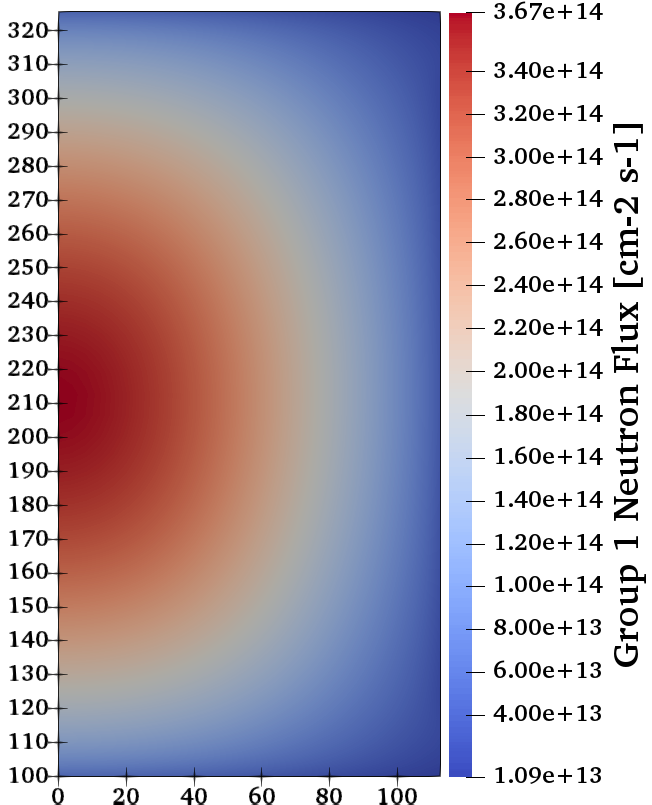
\includegraphics[width=\textwidth]{ss-g1}
    \end{subfigure}
    \begin{subfigure}[t]{.325\textwidth}
        \centering
        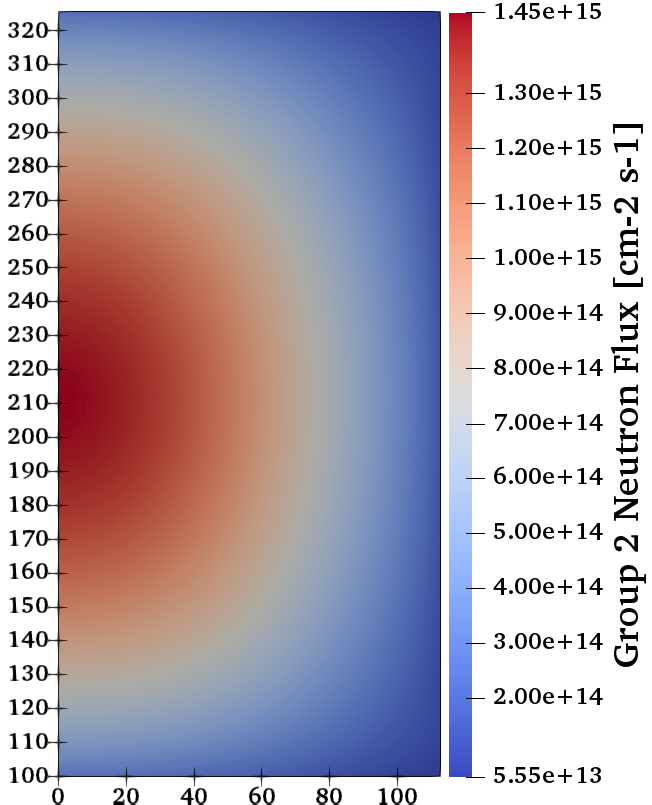
\includegraphics[width=\textwidth]{ss-g2}
    \end{subfigure}
    \begin{subfigure}[t]{.325\textwidth}
        \centering
        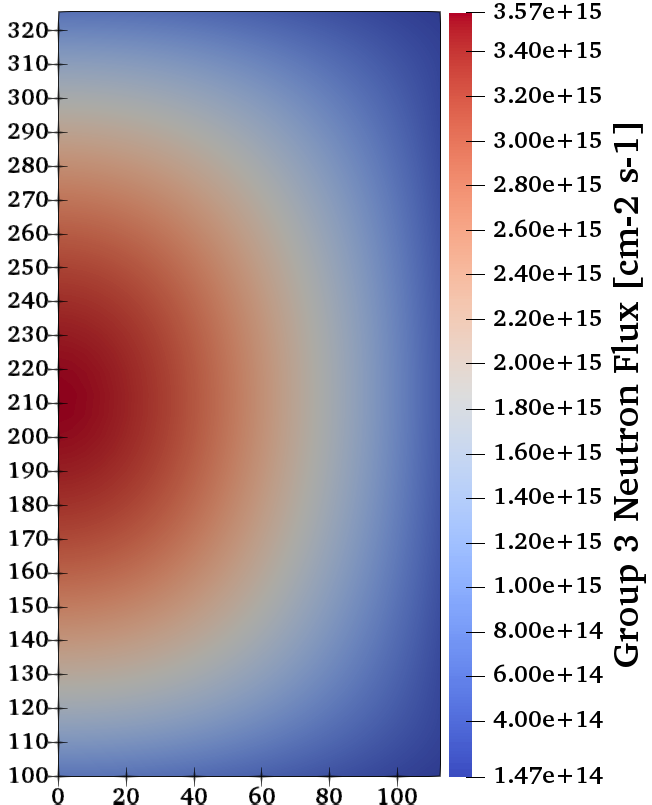
\includegraphics[width=\textwidth]{ss-g3}
    \end{subfigure}
    \begin{subfigure}[t]{.325\textwidth}
        \centering
        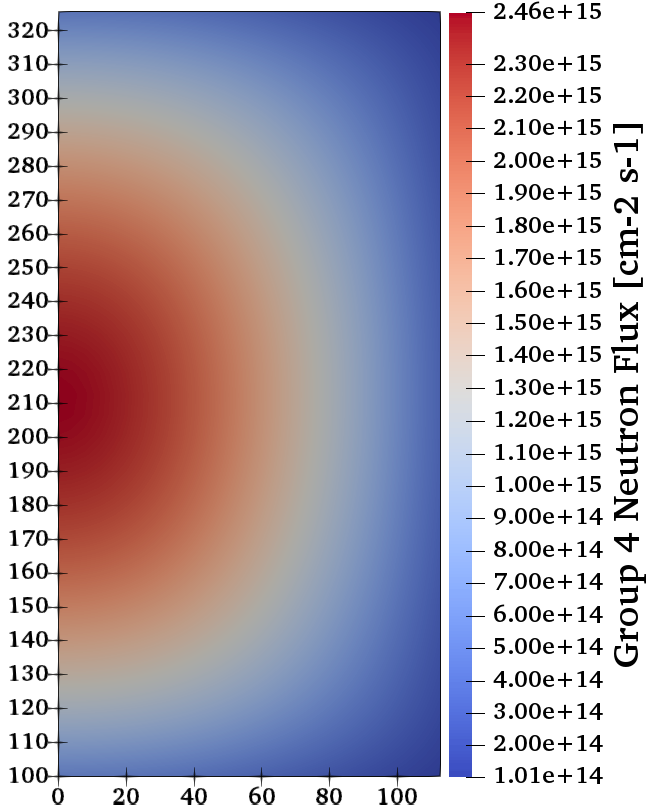
\includegraphics[width=\textwidth]{ss-g4}
    \end{subfigure}
    \begin{subfigure}[t]{.325\textwidth}
        \centering
        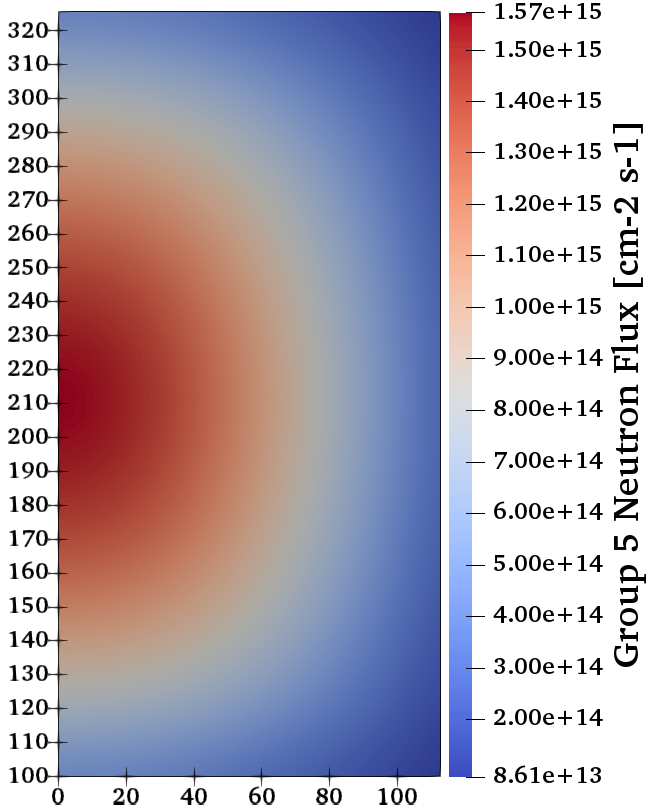
\includegraphics[width=\textwidth]{ss-g5}
    \end{subfigure}
    \begin{subfigure}[t]{.325\textwidth}
        \centering
        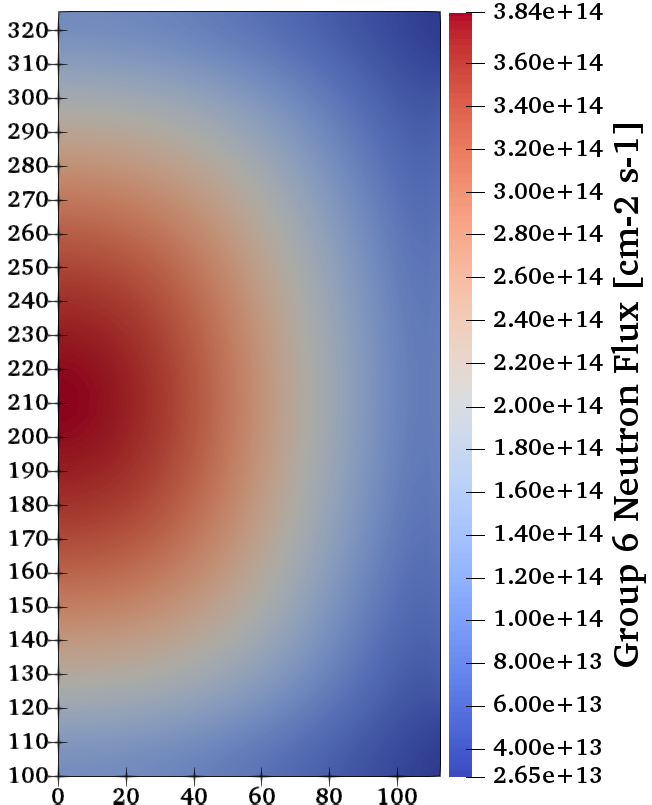
\includegraphics[width=\textwidth]{ss-g6}
    \end{subfigure}
    \caption{Neutron flux distributions in the core for neutron energy groups
    1 to 6. The y and x axes represent height and radius values of the core
    relative to the entire reactor geometry.}
    \label{fig:neutronflux}
\end{figure}

\begin{figure}[t!]
    \centering
    \begin{subfigure}[t]{.49\textwidth}
        \centering
        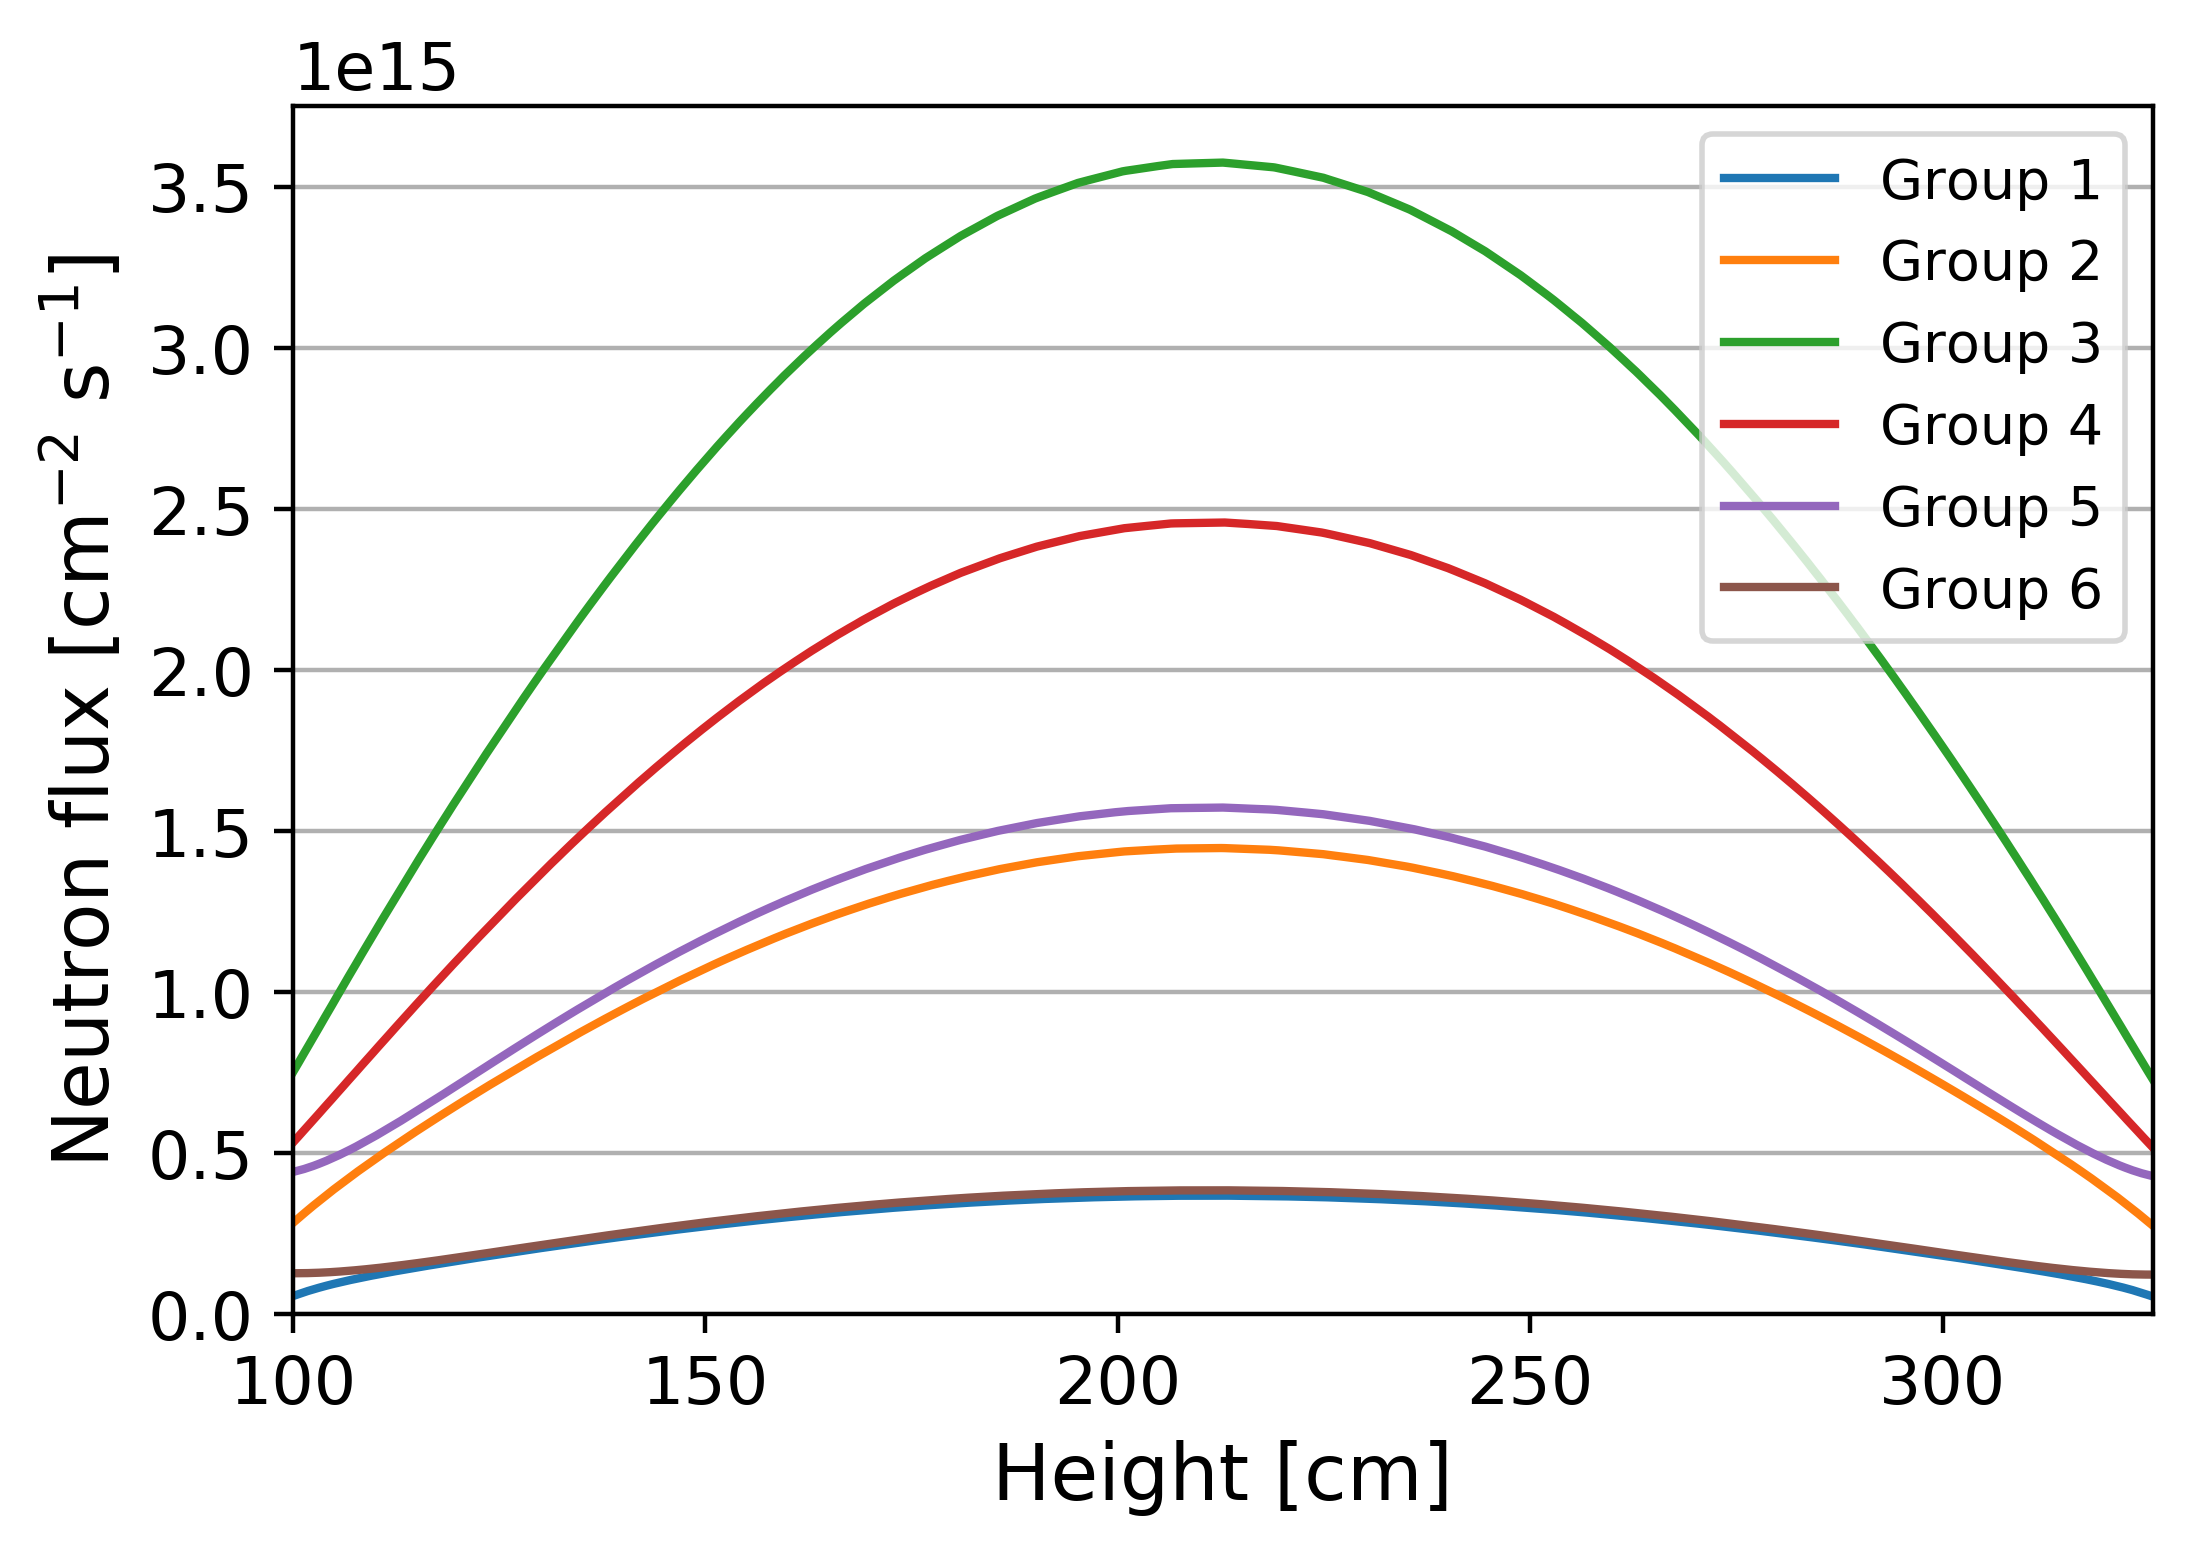
\includegraphics[width=\textwidth]{axial-flux}
    \end{subfigure}
    \begin{subfigure}[t]{.49\textwidth}
        \centering
        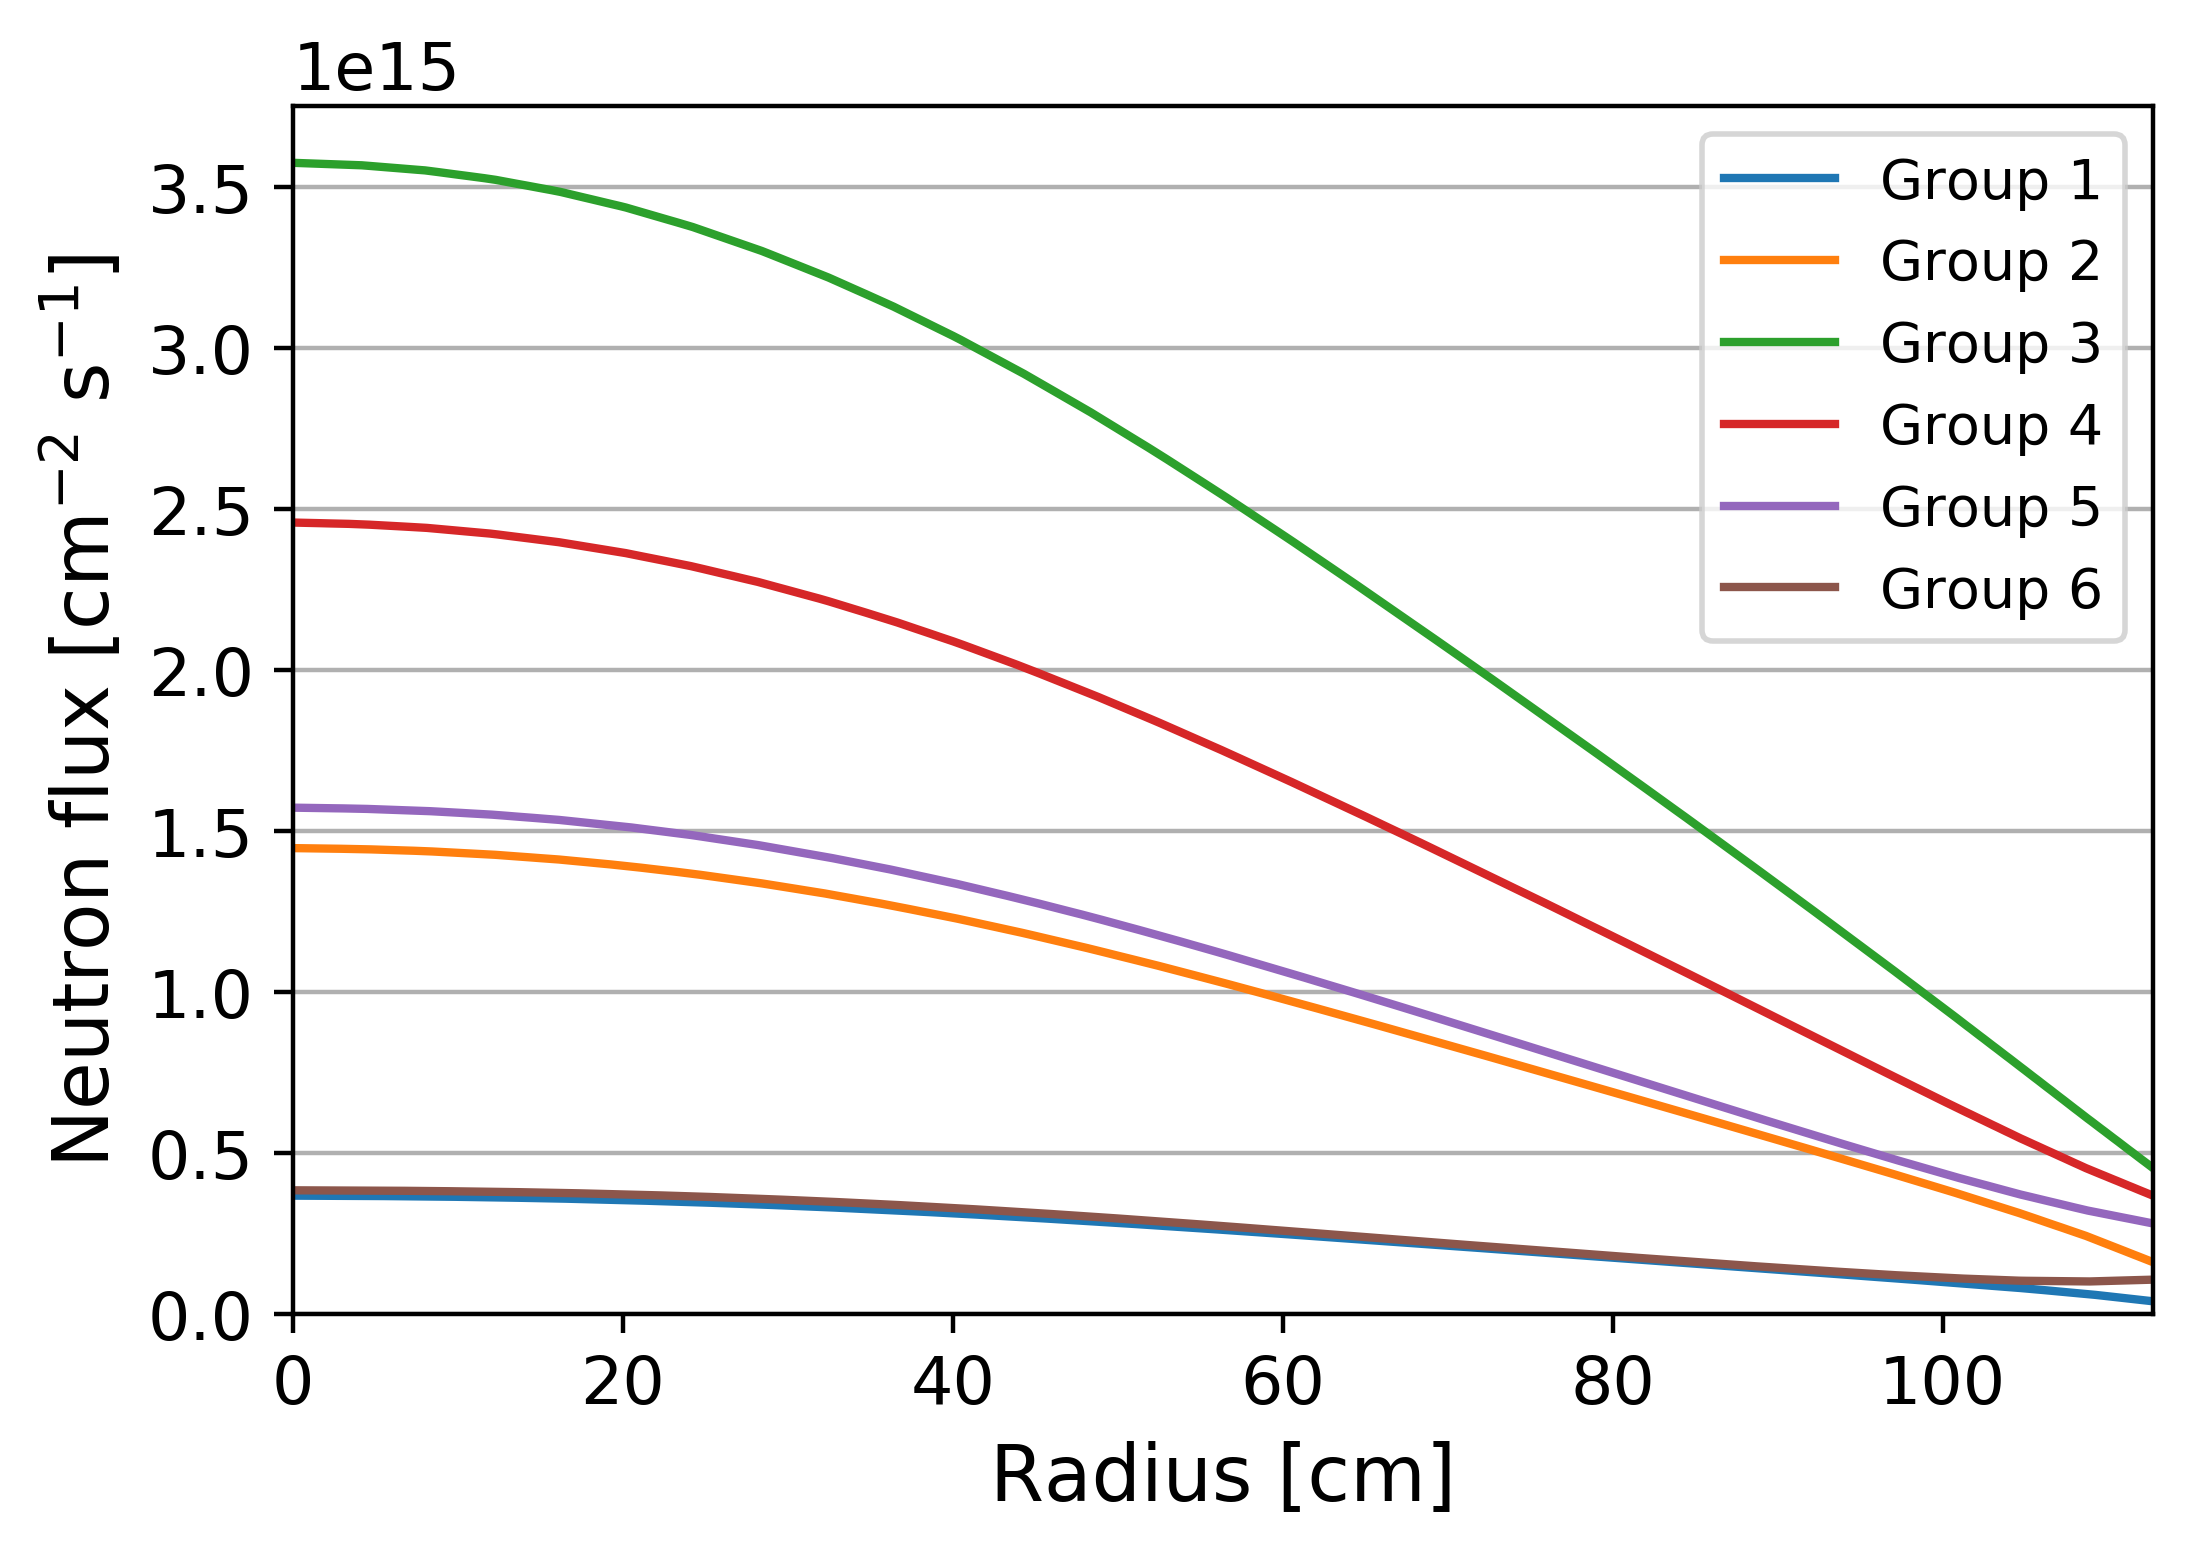
\includegraphics[width=\textwidth]{radial-flux}
    \end{subfigure}
    \caption{Axial (left) and radial (right) neutron flux distributions in the
    core for neutron energy groups 1 to 6.}
    \label{fig:axialradial}
\end{figure}

\begin{table}[t!]
	\centering
	\caption{Peak neutron flux values from Moltres (this paper), COMSOL
	\cite{fiorina_molten_2013}, and OpenFOAM \cite{aufiero_development_2014}
	models. The COMSOL and OpenFOAM values were calculated with uniform
	temperature distributions.}
	\begin{tabular}{l S}
		\toprule
		{Model} & {Peak Neutron Flux [$\times 10^{15}$ cm$^{-2}$ s$^{-1}$]}
		\\
		\midrule
		{Moltres (This paper)} & 9.80\\
		{COMSOL} & 8.6 \\
		{OpenFOAM} & 9.0 \\
		\bottomrule
	\end{tabular}
	\label{table:peak-flux}
\end{table}

As mentioned before, the \glspl{DNP} are mobile in \glspl{MSR} and their
distributions do not directly correspond to the neutron flux distributions.
The location where the \glspl{DNP} decay and emit neutrons impacts their
neutron
importance depending on their proximity to fissile and parasitic isotopes.
Figure \ref{fig:dnp} shows the \gls{DNP} distributions for all eight \gls{DNP}
groups. The
precursors from the shortest-lived group (Group 8) predominantly decay within
the core as their half-lives are shorter than the time it takes to reach the
outlet while the precursors from the longest-lived group (Group 1) are
effectively uniformly distributed due to their long half-lives relative to the
average circulation time. For the longer-lived groups, the mesh elements with
relatively high and low \gls{DNP} concentrations near the outlet and inlet,
respectively, suggest that the mesh is too coarse. Thus, we would recommend
further refinement for future work involving similar geometries.

\begin{figure}[htb!]
    \centering
    \begin{subfigure}[t]{.243\textwidth}
        \centering
        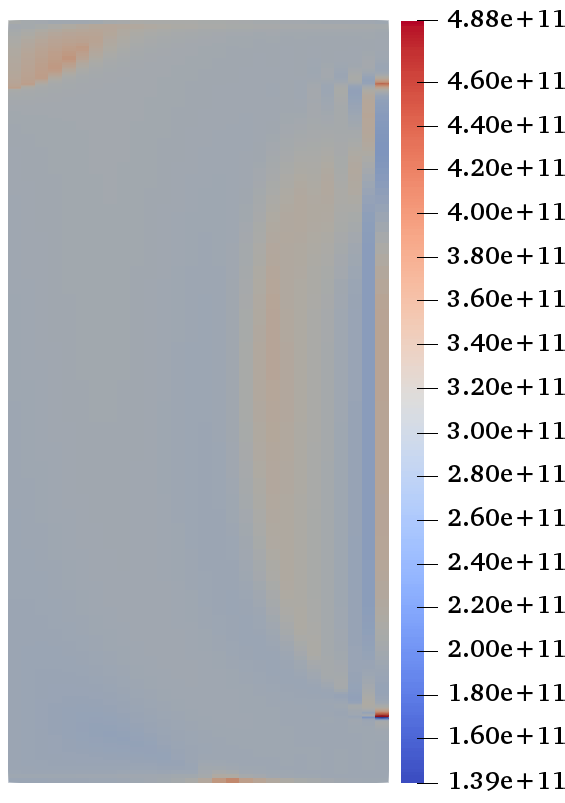
\includegraphics[width=\textwidth]{ss-pre1}
    \end{subfigure}
    \begin{subfigure}[t]{.243\textwidth}
        \centering
        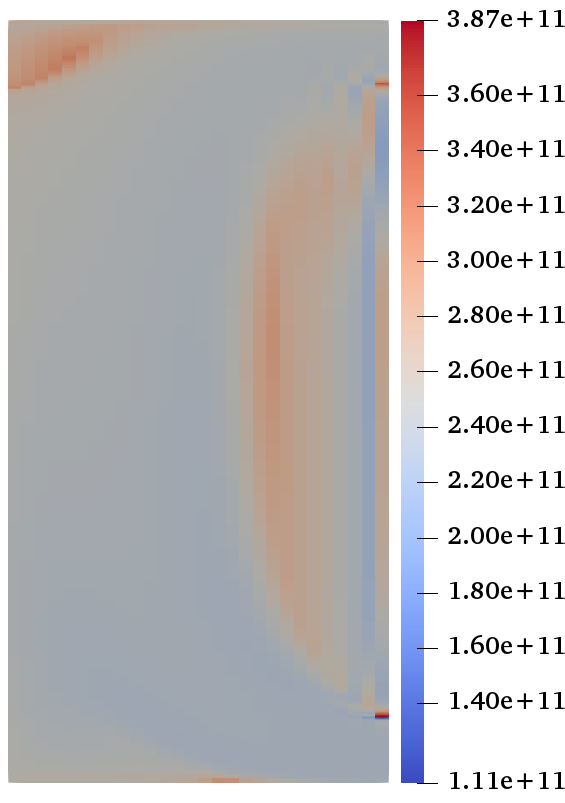
\includegraphics[width=\textwidth]{ss-pre2}
    \end{subfigure}
    \begin{subfigure}[t]{.243\textwidth}
        \centering
        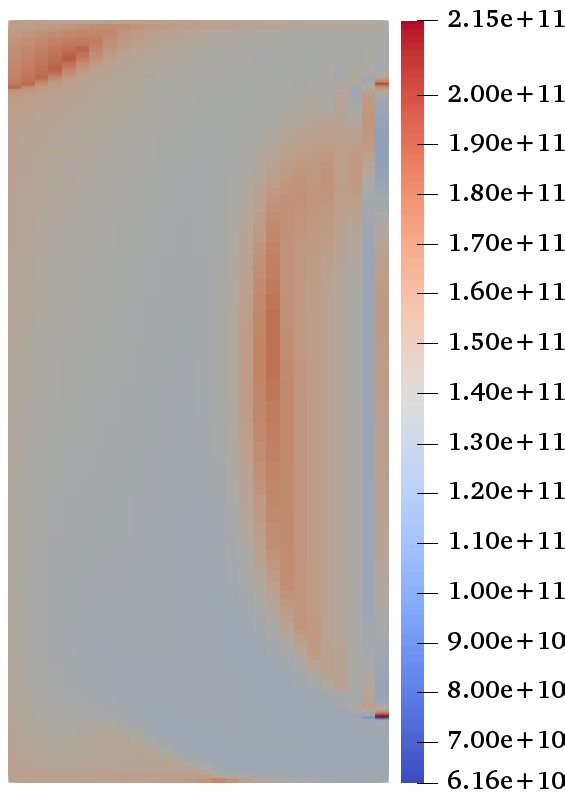
\includegraphics[width=\textwidth]{ss-pre3}
    \end{subfigure}
    \begin{subfigure}[t]{.243\textwidth}
        \centering
        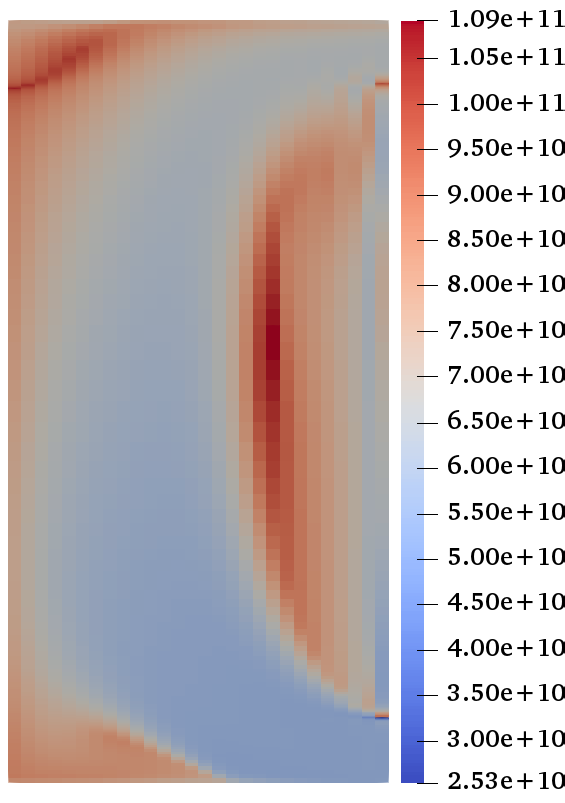
\includegraphics[width=\textwidth]{ss-pre4}
    \end{subfigure}
    \begin{subfigure}[t]{.243\textwidth}
        \centering
        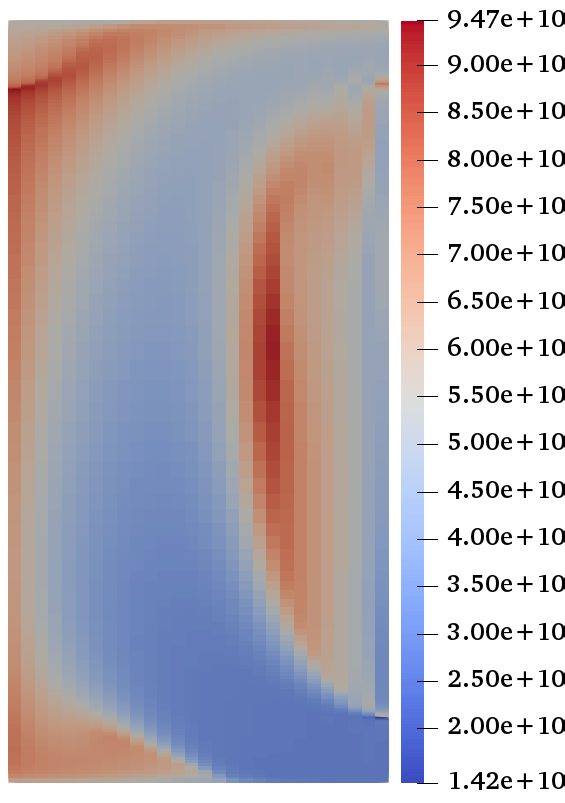
\includegraphics[width=\textwidth]{ss-pre5}
    \end{subfigure}
    \begin{subfigure}[t]{.243\textwidth}
        \centering
        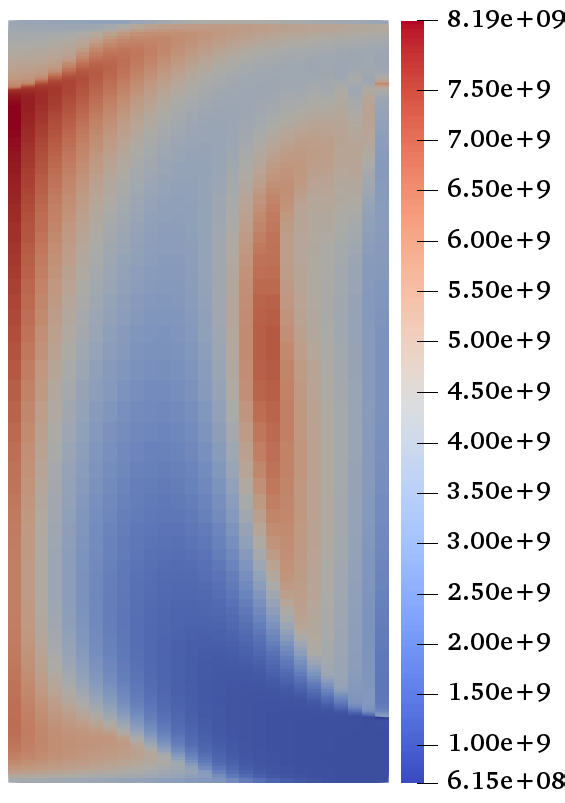
\includegraphics[width=\textwidth]{ss-pre6}
    \end{subfigure}
    \begin{subfigure}[t]{.243\textwidth}
        \centering
        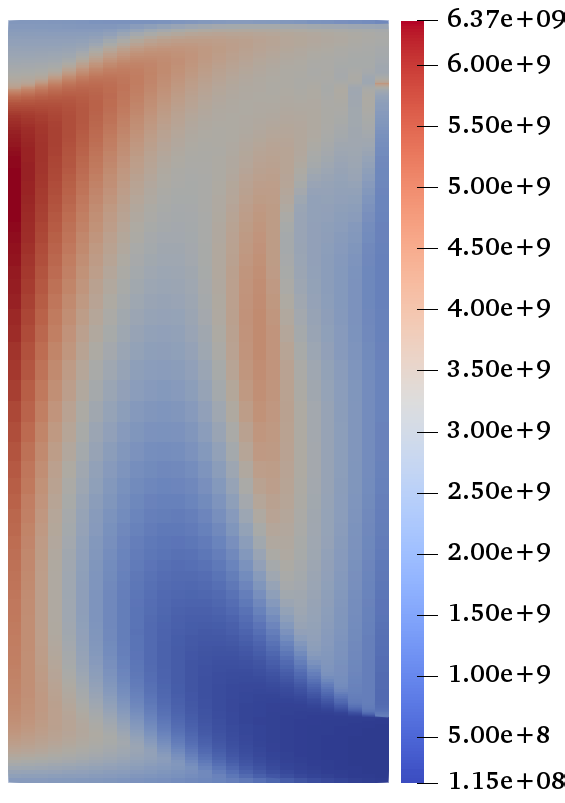
\includegraphics[width=\textwidth]{ss-pre7}
    \end{subfigure}
    \begin{subfigure}[t]{.243\textwidth}
        \centering
        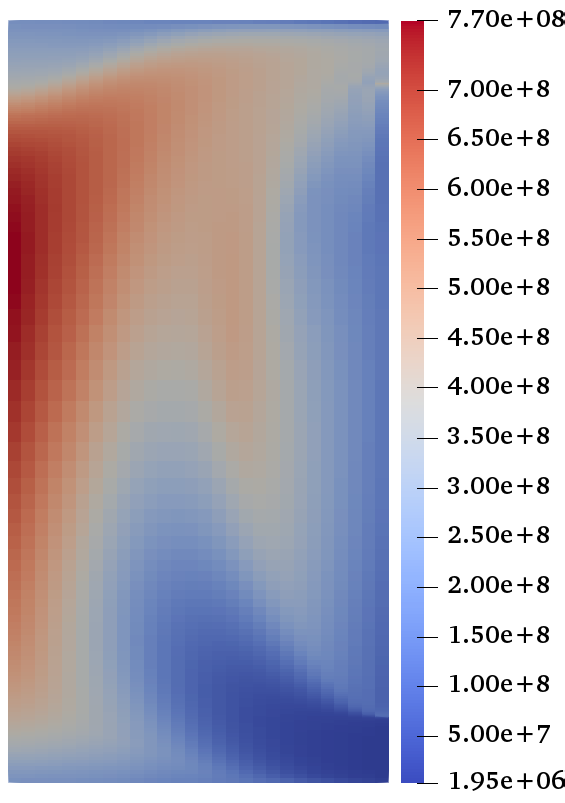
\includegraphics[width=\textwidth]{ss-pre8}
    \end{subfigure}
    \caption{\gls{DNP} distributions in the core for \gls{DNP} groups
    1 to 8 (from left to right, top to bottom). Refer to Figure \ref{fig:neutronflux} for the height and radius
    scales on the y and x axes, respectively. Note the different scales for
    each distribution.}
    \label{fig:dnp}
\end{figure}

\subsection{In-Core \texorpdfstring{$\beta_{\text{eff}}$}{beta_eff}}

An important safety parameter for \glspl{MSR} is the actual in-core
$\beta_{\text{eff}}$ value. This value represents the actual effective delayed
neutron fraction in \glspl{MSR} after accounting for the loss of delayed
neutrons due to out-of-core \gls{DNP} decay. Table * shows 

\section{Decay Heat}

The inclusion of a decay heat model effectively redistributes a fraction of
the volumetric heat source from the center of the core to the entire loop.
Thus, we expect to observe a slight flattening of the temperature distribution
across the entire primary loop.
